\subsection{Efficient and consistent data plane strategies}

\begin{task}
\label{task:system:dataplane}
We will design and implement efficient  data-plane implementations by extending  software-defined networking   
 techniques to  guarantee  reachability and consistency  
 properties in the presence of reconfiguration and link dynamics.
\end{task}


\begin{wrapfigure}{r}{0.4\textwidth}
\vspace{-0.4cm}
\centering
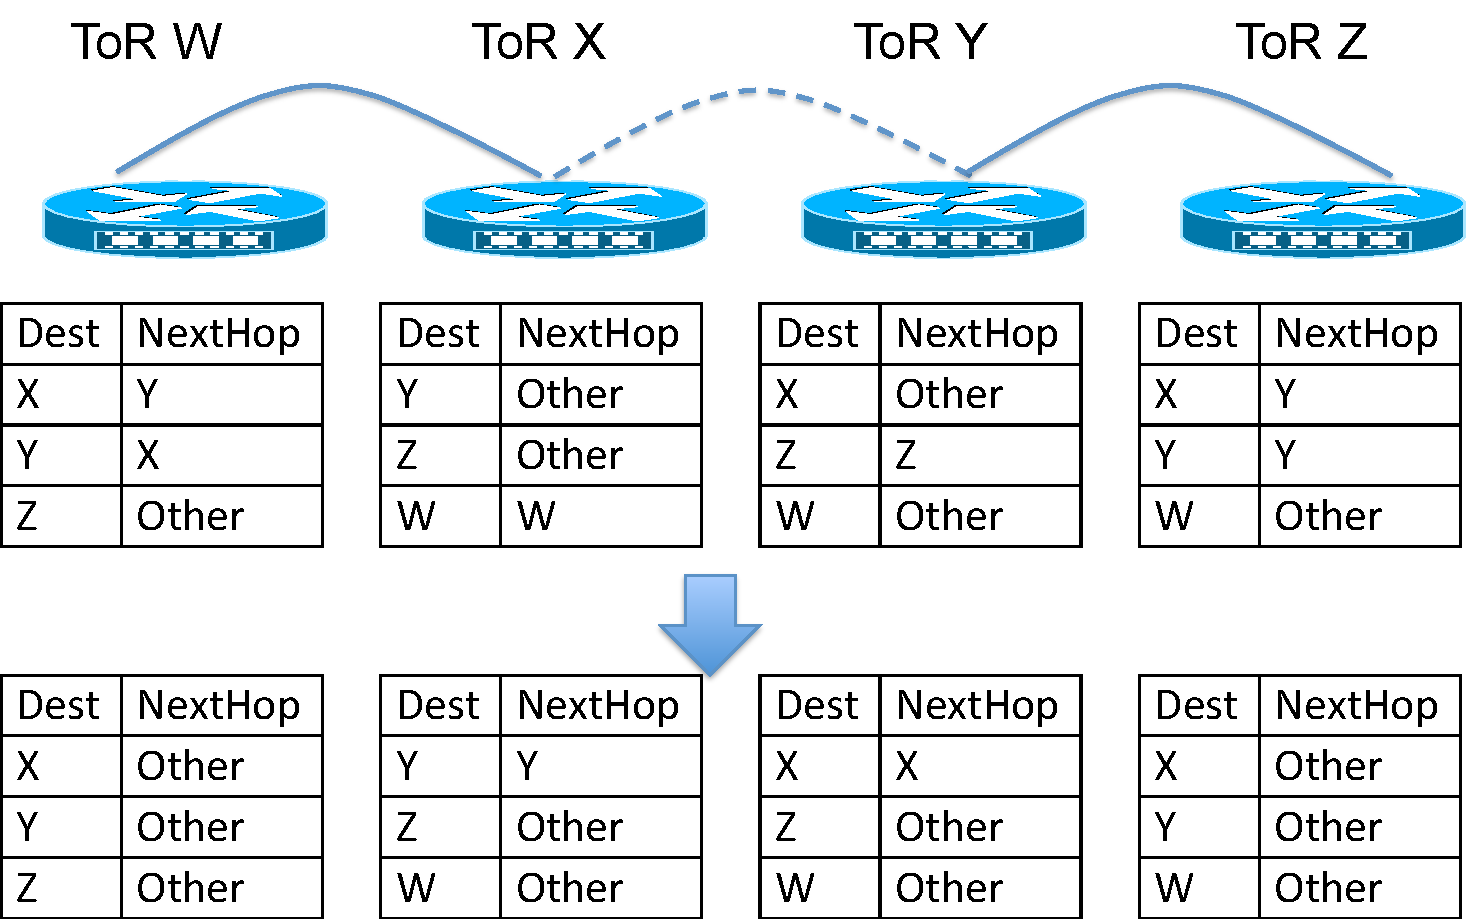
\includegraphics[width=200pt]{PPTFigs/consistency.pdf}
\caption{Example to illustrate the need for careful and consistent
routing management in \ArchName}
\label{fig:sys:cons}
\end{wrapfigure}


\mypara{Problem context} Our focus here is on translating the solution provided
by optimization engine into a practical data plane forwarding strategy. Here,
we leverage recent advances in software-defined networking (SDN)  to  implement
the topology and routing reconfiguration strategies~\cite{}.  While SDN is an
``enabler'' as  it provides cleaner management abstractions and open interfaces
(e.g., via APIs such as OpenFlow~\cite{}), \ArchName introduces  unique
efficiency, correctness, and consistency challenges during network
reconfigurations and local link readjustments. 




\eat
{
 SDN  is characterized by three key ideas: (1)
decoupling the ``control plane'' of the network from the ``data plane'' (e.g.,
avoiding embedding  the traffic engineering or access control policy into the
topology or routing algorithms); (2) a logically centralized management layer
that operates in the principle of ``direct control''; and (3) the use of open
APIs to configure the behaviors of data plane elements such as routers and
switches. The de-facto standard for SDN today is embodied in the design of the
OpenFlow protocol~\cite{}. Switches supporting OpenFlow export a simple  data
plane abstraction to the controller -- matching on specific ``flow'' header
fields and taking specific actions (e.g., forward, drop, count). This
``flowtable'' or the set of actions can be programmatically configured by a SDN
controller via the OpenFlow API.  In this respect, the \ArchName management
layer mirrors the SDN philosophy -- a logically centralized management module
that is reconfiguring  the topology and routing in response to workload
changes. The goal of our data plane translation layer is to translate the
optimization solution into a suitable set of forwarding rules compatible with
the  OpenFlow API. Thus, SDN is an obvious enabler for \ArchName -- it is quite
 challenging (and possibly infeasible) to realize such the fine-grained topology and
traffic engineering  we required   on top of traditional routing protocols. 
}


%\begin{packeditemize}
%First, the network topology is constantly
%in a state of flux and will be actively modified by the controller. In
%contrast, most SDN work treats the topology as a ``read-only'' object
%that only changes on coarse timescales.  



\noindent {\em Network reconfigurations:} Consider the scenario in
Figure~\ref{fig:sys:cons}, where \ArchName is reconfiguring the network
topology and we want to active the X-Y link and disable X-W and Y-Z. The
problem here is that during the  reconfiguration, tables of the switches may
have an inconsistent view of the topology.  For instance, if we update the
forwarding tables to use the X-Y link before the link is active or conversely
if we do not update the routes to disable routes using Y-Z or X-W, then we may
have connectivity issues.   Furthermore, if there were large elephant flows 
using the Y-Z or X-W links, then moving them may cause transient congestion in 
  other parts of the network and impact their completion times. 

Our goal is to ensure that even during this transient periods, packets are not
dropped; we get reasonable performance; and there are no adverse effects due to
forwarding loops. While this seems  related to work on {\em consistent
updates}\footnote{This guarantees that each packet is either processed by an
old configuration or a new configuration but not a mix.} in
SDN~\cite{consupdate,incconsupdate}, this is indeed a useful theoretical
framework, there are two unique challenges.  First, this prior work implicitly
assumes that the network topology has not changed between the two update
states---in \ArchName, the topology might itself may change.  Second, it does not 
provide guarantees on the bandwidth or the throughput during the transition
period~\cite{caesarhotsdn12}.  


\noindent {\em Link flux:} Second, even with a static topology state, links may
be transiently unavailable because of the ``micro alignment'' that each FSO
device may need  to  run.  The timescales of such micro-alignment may be much
smaller than the time needed to communicate with an SDN controller and waiting
for rule updates~\cite{ddcnsdi13}. In fact, it may be counterproductive to
report such transient link failures to the controller as it may cause needless
topology reconfigurations. Thus, in addition to the link micro-alignment
mechanisms discussed in Section~\ref{sec:fso}, we also need corresponding
network layer techniques.

% to utilize this information.

%the nature of the
%FSO-based link-layer technologies in \ArchName may introduce very fine
%timescale link unreliability issues that warrant mechanisms that need
%{\em local recovery} mechanisms that  possibly cannot involve the
%controller.



%\end{packeditemize}

%To see why dynamic topology changes   might cause problems, 


%Finally, it
%effectively requires double the ``rule space'' on the network switches
%to hold both sets of forwarding rules.


%Thus, we need mechanisms to ensure that the 


%While the general problem of reasoning about 
%resource utilization in a consistent update model is quite hard~\cite{}, 
 % Rather than solve the general problem of resource utilization and local
%recovery, we plan to explore domain- and problem-specific strategies. 
\mypara{Proposed approach}  We believe it is useful to decouple the
three types of requirements: {\em connectivity during reconfigurations},
{\em connectivity during link realignment},  and {\em performance} as
these entail different solution strategies. Corresponding to these requirements, 
we will explore three techniques: 

\begin{packeditemize}
\item {\em Guaranteeing reachability during reconfigurations:} We will explore
approaches to  guarantee end-to-end reachability even in the presence of
topology reconfigurations. For instance, we will set aside a subset of the
\InterRack links to be ``always on'' (or statically aligned)  to create a
connected ``backbone'' (e.g., a spanning tree) to ensure that  all pairs of
racks can always reach other. By itself, a backbone does not guarantee data
plane reachability, and we need to {\em carefully schedule} the reconfiguration
operations.  %\item {\em Careful scheduling:} 

 Consider the earlier example from Figure~\ref{fig:sys:cons}.  The key here is
in the ordering of the steps---we remove routes before deactivating links and
add routes only after activation is complete in the following sequence: (1)
Update routing table to reflect the removal of  links $(x,w)$ and $(y,z)$; (2)
Switch the FSO links to activate/deactivate links; and (3) When (2) is
complete, we update routing tables to reflect the addition of link $(x,y)$.  We
believe this intuition can be extended to the multiple reconfiguration case as
well by a combination of suitable batching and parallelization strategies
(e.g., find non-conflicting scenarios.)  

\item {\em Handle link flux locally:} Future SDN roadmaps have provisions for local recovery
mechanisms analogous to similar schemes in the MPLS and SONET
literature~\cite{}. We will explore the available alternatives for our
prototype implementation.  In the absence of such features, we will explore the
possibility of running a local ``lightweight'' SDN controller on every rack
that can quickly react to the micro-alignment changes but relies on the global controller for
longer-timescale reconfigurations~\cite{ddc}.

%s discussed earlier,
%existing consitent update abstractions do not provide mechanisms to reason
%about the resource usage. 

\item {\em Minimizing impact of  reconfigurations:}  In order to minimize the
impact of a reconfiguration  on  network congestion, we can extend the
optimization from \taskref{task:sys:fastalgo} and additional objective criteria
(or constraints) that will force the optimizer to  prefer  reconfigurations
that cause minimal disruption for the active ``elephant'' demands.  Because
\ArchName has more degrees of topological freedom relative to prior work, we
may be able to minimize disruptions for existing connections by simply
introducing additional links on-demand.

%Again, we believe that the enhanced 
%flexibility that  \ArchName  offers has a natural synergy. .
 
\end{packeditemize}
 

\eat
{
\vyas{this is a dump of older thoughts.. no structure yet.}

\begin{itemize}

\item system -- collects TM info, collects link status info, computes the topology/routing, 
 reconfigures the routing rules

\item assume algo "speed" been addressed in the previous topology section? else fast/incremental computation goes here..

\item when to reconfigure -- periodic + triggered by large deviations in TMs -- probably 
 dont want to do this too often -- need some way to determine if changing gives enough 
 benefits?

\item we need some way to globally monitor  per fso-link  link status and do 
 micro-alignments .. and track these so these links are not used while they are down?

\item how do you quickly reconfigure a large network? with several hundred switches?

\item how do you guarantee consistency of paths, loop-free-ness, reachability
etc during such an update?

\item how can we cleanly partition/scale this controller .. likely one server is not 
going to suffice .. this ties in to the consistency problems ?

\item  need some large-scale monitoring framework to track the traffic matrix, 
 elephant flows etc .. do this with low overhead and high fidelity somehow

\item is there way to compact-ify the rules? may not have enough rule space

\item do we need some link-local recovery mechanism because centralized will not work? e.g., look 
 at DDC or other solutions?

\item are we doing in-band or out-of-band control here? if in-band then we have another problem that we may not have a way to get the link status info itself to the controller? 


\end{itemize}
}
